

\section{Cluster algorithms}
\label{sec:cluster_algorithms}


We have seen that the larger our system is, the longer we have to wait to sample our states. This happened because just flipping one or a few spins before sampling ends up in a strong correlation between the states, and the assumption of statistically independent samples is not given anymore. The aim of cluster algorithms is to reduce this critical slowing down by flipping multiple spins. It is essential that the group of spins to flip is chosen with a tiny acceptance probability. To do this, we will generalize the Ising model and adapt it to our needs.

 
\subsection{Potts Model}
The Potts model is a generalization of the Ising model to a $q$-states model, and it also exhibits in certain cases a first order phase transition at a critical temperature. Applications of the Potts model range from sociology through biology to material science, making this a very versatile model. The Potts model exhibits a first order transition in 2D for any $q$ larger than 4, and for any $q$ larger than 2 for dimensions larger than 2. We start by defining the Hamiltonian of the system as
\begin{equation}
\mathcal{H} = -J\sum_{i,j=nn} \delta_{\sigma_i,\sigma_j} - H_1\sum_{i} \delta_{\sigma_i,\sigma_1}
\label{eq:potts_model}
\end{equation}
with $\sigma_i \in \mkl{1,...,q}$, and $q$ being an integer $\geq 2$. In this case, the state ``1'' is favored, by lowering the energy whenever a site is in this particular state. The sites of the lattice we are dealing with can assume more than just two states (up/down, as we had in the Ising model). The interesting fact now is that there is a strong connection between the Potts model and the well known bond percolation model. After Kasteleyn and Fortuin (1969), which we will discuss now, the two models have related partition functions. 


\vspace{0.1cm}
\noindent
\noindent\begin{minipage}{\textwidth}
\begin{minipage}{.98\textwidth}
  \centering
  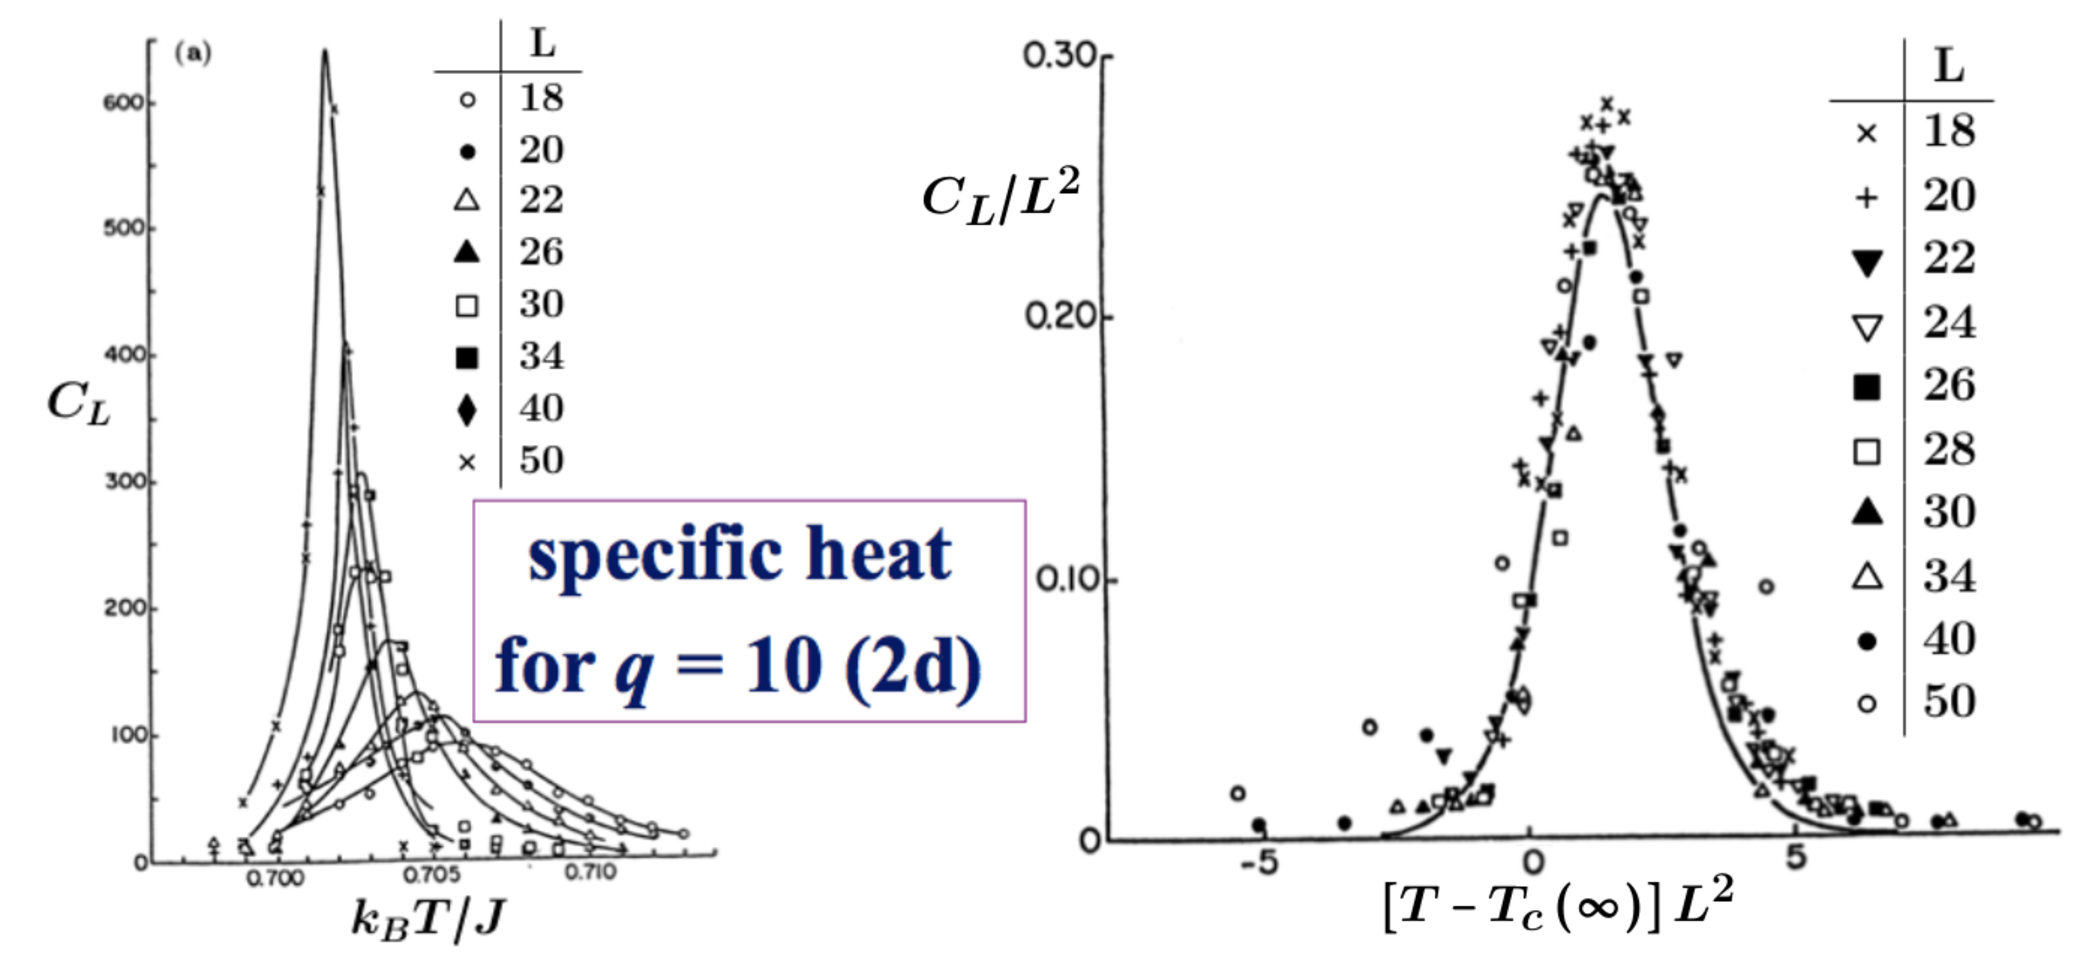
\includegraphics[width = 0.95\textwidth]{pics/potts10}
  \captionof{figure}{Specific heat for two dimensional Potts model with q=10. On the right the scaling for different sizes.}
  \label{fig:potts10}
\end{minipage}\hfill
\end{minipage}
\vspace{0.1cm}

Any system is characterized by its partition function. From the latter one can derive all other thermodynamic quantities. Therefore the complete knowledge of the partition function corresponds to the complete knowledge of the system. If two systems have exactly the same partition function, those two systems are therefore equivalent. In the following, we will prove a relation between the bond percolation and the Potts model.


\subsubsection*{The Kasteleyn and Fortuin theorem:}
Consider the Potts model not on a square lattice, but on an arbitrary graph of nodes connected with bonds. On the nodes we have $q$ possible states, and for every connection we have an energy cost of 1 if two connected nodes are in a different state and of 0 if they are in the same state.
\begin{equation}
E= J \sum_\nu \epsilon_\nu \hspace{1cm} 
\text{with }
\epsilon_\nu =\begin{cases}
  0  & \text{if endpoints are in the same state }\\
  1 & \text{else }
\end{cases}
\label{eq:energy_potts}
\end{equation}

We also introduce two operations on the bonds: the \emph{contraction C} and \emph{deletion D} (see Fig. \ref{fig:contr_del}). Bonds can thus be either removed by merging two sites (which implies that they have the same state) or be simply removed.

  \begin{center}
  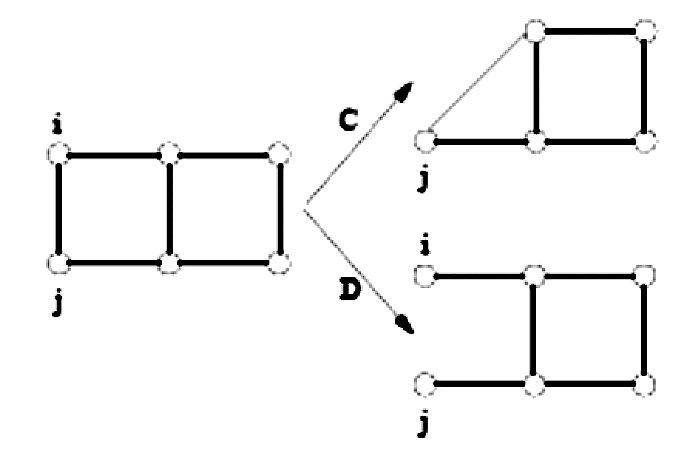
\includegraphics[width = 0.7\textwidth]{pics/contr_del}
  \captionof{figure}{Contraction and deletion of bonds.}
  \label{fig:contr_del}
\end{center}
\vspace{0.1cm}

\begin{comment}
\vspace{0.1cm}
\noindent
\noindent\begin{minipage}{\textwidth}
\begin{minipage}{.48\textwidth}
We also introduce two operations on the bonds: the \emph{contraction C} and \emph{deletion D} (see Fig. \ref{fig:contr_del}). Bonds can thus be either removed by merging two sites (which implies that they have the same state) or be simply removed.
\end{minipage}\hfill
\begin{minipage}{.48\textwidth}
  \centering
  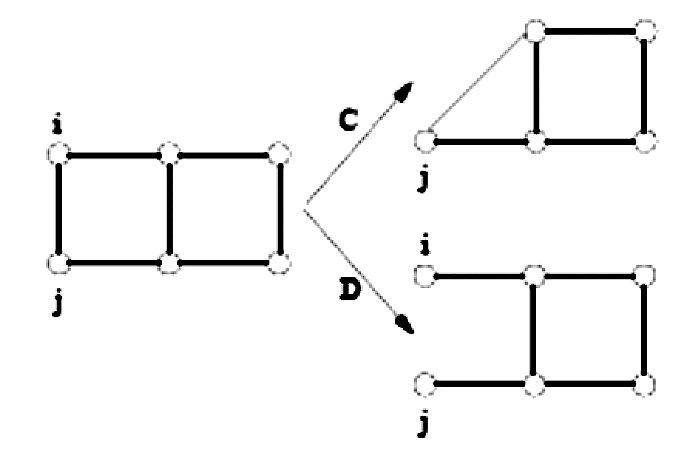
\includegraphics[height=150pt]{pics/contr_del}
  \captionof{figure}{Contraction and deletion of bonds.}
  \label{fig:contr_del}
\end{minipage}
\end{minipage}
\vspace{0.1cm}
\end{comment}

The partition function is the sum over all the possible configurations weighted by the Boltzmann factor:
\begin{equation}
Z=\sum_X{      e^{    -\beta E\kl{X}    }       } 
\overset{\text{\eqref{eq:energy_potts}}}{=} 
\sum_X{e^{-\beta J \sum_\nu {\epsilon_\nu}}} =
\sum_X   \prod_\nu{e^{-\beta J\epsilon_\nu}} 
\end{equation}
We will now consider a particular bond $\nu_1$ and rewrite the partition function as
\begin{align*}
\sum_X  e^{-\beta J\epsilon_{\nu_1}} \prod_{\nu\neq\nu_1}{e^{-\beta J\epsilon_\nu}} &=
\sum_{X,\sigma_i =\sigma_j}  \prod_{\nu\neq\nu_1}{e^{-\beta J\epsilon_\nu}} + e^{-\beta J} \sum_{X,\sigma_i\neq\sigma_j}  \prod_{\nu\neq\nu_1}{e^{-\beta J\epsilon_\nu}} \\
& =Z_C + e^{-\beta J} \kl{Z_D - Z_C}\\
& = \kl{1 - e^{-\beta J\epsilon_\nu}} Z_C + e^{-\beta J}Z_D\\
&= p Z_C + \kl{1-p} Z_D
\end{align*}
Here $\sigma_i$ and $\sigma_j$ are the states at the two ends of the bonds, $Z_C$ and $Z_D$ are the partition functions of the graphs contracted and deleted at $\nu_1$ respectively and $p\equiv1-e^{-\beta J}$ . We have now divided the partition function in a sum of two other partition functions, namely the partition function of the same system with a deleted bond and the partition function of the same system with a contracted bond. We can repeat this operation on another bond $\nu_2$, and we find that
$$
Z = p^2Z_{C_{\nu_1},C_{\nu_2}} + p(1-p) Z_{C_{\nu_1},D_{\nu_2}} + (1-p)^2 Z_{D_{\nu_1},D_{\nu_2}}.
$$
We repeat this operation on every bond. At the end the graph is reduced to a set of separated points corresponding to connected/contracted bonds: the clusters of sites which are connected and in the same state. The partition function is then reduced to:
\begin{equation}
Z= \sum_{\underset{\text{{ bond percolation}}}{\text{ \fontsize{6.5}{4}\selectfont configuration of}}} {q^{\text{\# of clusters}} p^c \kl{1-p}^d}
= \avkl{q^{\text{\# of clusters}}}_{\text{bond percolation configurations}}
\label{eq:part_func_coniglio}
\end{equation}
where $c$ and $d$ are the numbers of contracted and deleted bonds respectively. We have now an equivalence between a purely geometrical model (percolation) and a thermal (or magnetic) model with a Hamiltonian (Potts model). Interestingly, one could now choose values for $q$ which are not integers. This made no sense in the beginning since $q$ was introduced as the state of each site. 

\subsubsection*{Coniglio-Klein clusters:}
Mind that the equivalence between the bond percolation model and the magnetic model is of statistical nature, since a particular bond configuration can have several spin configurations and a particular spin configuration can have several bond configurations. The fact that the value of the spins is absent in Eq. \eqref{eq:part_func_coniglio} forms the base for cluster algorithms. The probability of a given cluster $C$ to be in a certain state $\sigma_0$ is independent of the state itself:
\begin{equation}
p(C,\sigma_0) = p^{c_C}(1-p)^{d_C}  \sum_{\underset{\text{{ without cluster C}}}{\text{ \fontsize{6.5}{4}\selectfont bond percolation}}} {q^{\text{\# of clusters}} p^c \kl{1-p}^d}
\end{equation}

This means that flipping this particular cluster won't affect the partition function (and therefore the energy) so that it is possible to accept the flip with probability one. This can be seen by looking at the detailed balance for this system:
\begin{equation}
p(C,\sigma_1)W\ekl{(C,\sigma_1)\rightarrow (C,\sigma_2)}
=
p(C,\sigma_2)W\ekl{(C,\sigma_2)\rightarrow (C,\sigma_1)}
\end{equation}
and remembering that $p(C,\sigma_1)=p(C,\sigma_2)$. If we now apply Glauber dynamics we obtain $W=\frac{p(C,\sigma_2)}{p(C,\sigma_1)+p(C,\sigma_2)}=\frac{1}{2}$ and  $W=min\ekl{1,\frac{p(C,\sigma_2)}{p(C,\sigma_1)}}=1$ for Metropolis. This makes the cluster algorithm much faster than single-spin flip algorithms and reduces the problem of critical slowing down.

\subsection{O(n) Model}
There are a number of models that resemble the Ising model, but with slight modifications to adapt them to a particular context (e.g., the antiferromagnetic models, Ising spin glass, ANNNI model, metamagnets, ...). One of the possible generalizations of the Ising model is the so called n-vector model. Unlike the Potts model, it takes into account that the degrees of freedom of the sites do not have to be discrete. This is a very important model for describing phenomena related to magnetism (e.g., ferromagnetism). The variables on the sites are n-dimensional vectors. The Hamiltonian resembles the one of the Potts model in the sense that it favors alignment of the variables:

\begin{equation}
\mathcal{H} = J \sum_{i,j: nn} {\vec{S}_i \cdot \vec{S}_j } + H_1\sum_{i} { \vec{S}_i^1} 
\text{  \hspace{0.1cm}  with  \hspace{0.1cm} }
\vec{S}_ i= \kl{S_i^1,S_i^2,...,S_i^n} 
%\text{ \hspace{0.04cm} and  \hspace{0.04cm} }
\text{  and   }
\abs{\vec{S}_ i}= 1
\label{eq:antiferromagnetic}
\end{equation}
For $n=1$ we retrieve the Ising model, for $n=2$ we have the \emph{XY-model}, for $n=3$ the \emph{Heisenberg model} and finally, for $n=\infty$ we have the \emph{spherical model}.

Note that the models for various values of $n$ are not equivalent. In fact, there are huge differences. As an example, the XY-model does not exhibit any phase transition from an ordered to a disordered state. The proof of this statement can be found in \citet{mermin}, and it is known as the Mermin-Wagner theorem. Ernst Ising himself proved in his PhD thesis that the one dimensional case also does not exhibit any phase transition. In three dimensions, however, there are phase transitions and the behavior regarding magnetization, susceptibility and specific heat is very similar to the behavior of the Ising model we studied earlier (critical temperature, critical exponents etc.). 

For Monte Carlo simulations with continuous degrees of freedom we have to adapt our techniques because phase space is not a discrete set of configurations anymore. The classical strategy is to make spin flips by modifying the spin locally by a fixed amount (a rotation): $\vec{S}_i'=\vec{S}_i +\Delta \vec{S} $. The classical Metropolis algorithm can then be used in the same fashion as in the discrete models. In order to use cluster methods one can project a group of spins onto a plane, and then reflect the spins with respect to the plane.

In order to obtain clusters one has to find a method to identify ``equal'' spins. The probability to find equal spins in a continuous model vanishes and one can therefore considers a certain range of values instead(if two spins are equal within a certain error, then they belong to the same cluster).

\vspace{0.1cm}
\noindent
\noindent\begin{minipage}{\textwidth}
\begin{minipage}{.49\textwidth}
  \centering
  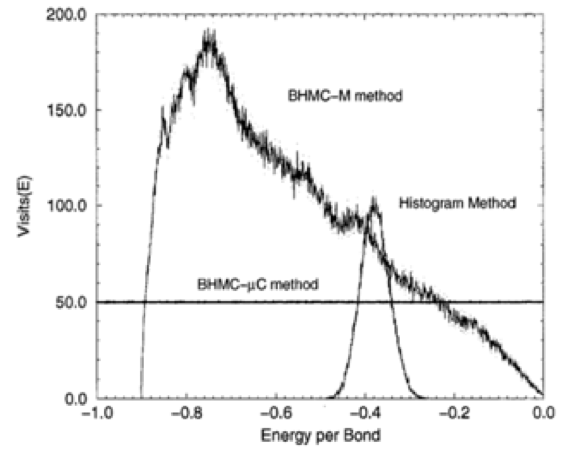
\includegraphics[height=170pt]{pics/en_bond}
 % \captionof{figure}{}
  \label{fig:en_bond}
\end{minipage}\hfill
\begin{minipage}{.49\textwidth}
  \centering
  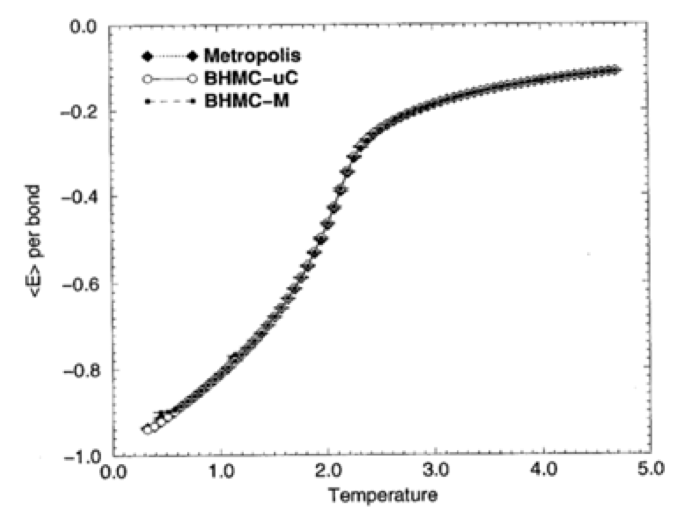
\includegraphics[height=170pt]{pics/e_xy}
  %\captionof{figure}{Number of visits done in the phase space against the energy.}
  \label{fig:e_xy}
\end{minipage}
\end{minipage}
\vspace{0.1cm}



\vspace{0.1cm}
\noindent
\noindent\begin{minipage}{\textwidth}
\begin{minipage}{.99\textwidth}
  \centering
  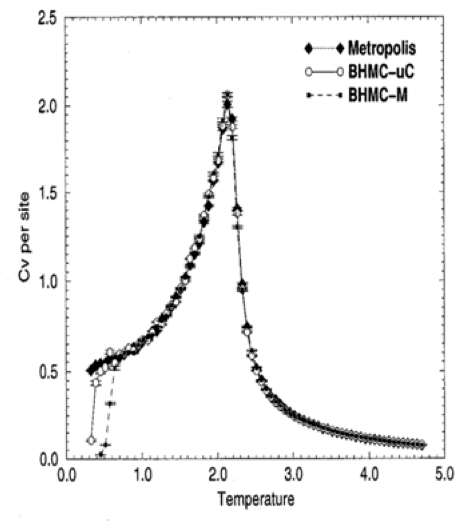
\includegraphics[height=260pt]{pics/cv_xy}
 % \captionof{figure}{}
  \label{fig:cv_xy}
\end{minipage}
\center
Figures: Broad Histogram method for the 3D XY model.
\end{minipage}



\subsection{Implementation of Cluster Algorithms}

\subsubsection*{Swendsen-Wang algorithm:}

The Swendsen-Wang algorithm is a refined Monte Carlo technique. For a certain configuration, we look through the bonds connecting the spins. Whenever two bonded sites  are in the same state, the two sites belong to the same cluster with probability $p\equiv 1-e^{-\beta J}$. Once the clusters are determined, they can be flipped using any of the dynamics mentioned above. The basic procedure is as follows:
\begin{itemize}
\item Occupy the bonds with probability $p\equiv 1-e^{-\beta J}$ if sites are in the same state.
\item Identify the clusters with the Hoshen-Kopelman algorithm.
\item Flip the clusters with probability 0.5 for Ising or choose always a new state for $q>2$.
\item Repeat the procedure.
\end{itemize}

\vspace{0.2cm}

\noindent\begin{minipage}{\textwidth}
\begin{minipage}{.98\textwidth}
  \centering
  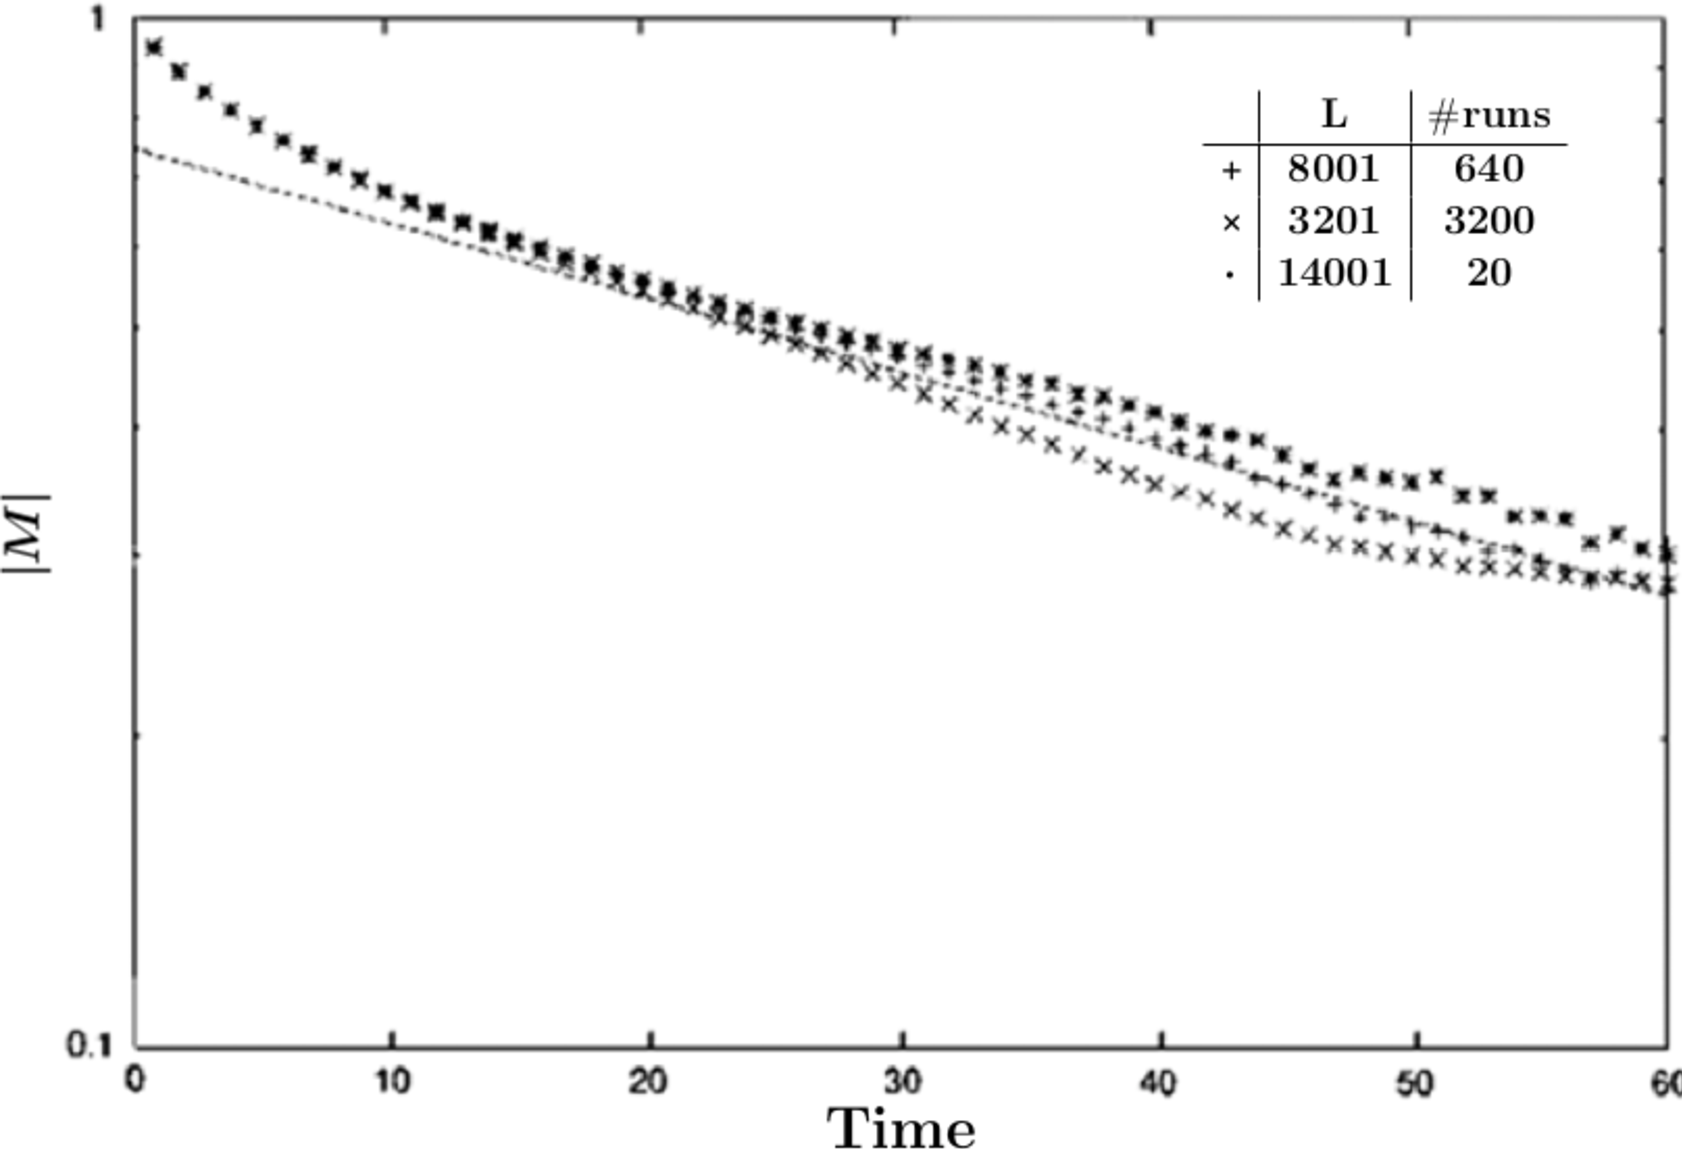
\includegraphics[width = 0.8\textwidth]{pics/critical_slowing_down_swendsen}
  \captionof{figure}{Critical slowing down for the Swendsen-Wang algorithm.}
  \label{fig:critical_slowing_down_swendsen}
\end{minipage}
\end{minipage}

\subsubsection*{Wolff algorithm:}
In this variant only one cluster is flipped per step using the \emph{Leath algorithm}:

\begin{itemize}
\item Choose a site randomly.
\item If neighboring sites are in the same state, add them to the cluster with probability $p\equiv 1-e^{-\beta J}$.
\item Repeat this for any site on the boundaries of the cluster, until all the bonds of the cluster have been checked exactly once.
\item Choose any new state for the cluster.
\item Repeat the procedure.
\end{itemize}
